\chapter{Localization system implementation}

\label{Chapter4}

In order to develop and evaluate the system outlined in Chapter \ref{Chapter3}, it is first required to establish a testing environment.
This chapter introduces the \red{technical} implementation of the localization system in a test bed.

\section{System Overview}

The test bed consists of multiple AN, a MN and a computer.

The ANs are commercial WiFi access pints, which are placed in the \red{area of interest} and constantly broadcast a beacon signal.

The MN, an android smartphone, is used to collect samples form different location in the area of interest. 

The collected samples are transferred to the computer where the calculations and algorithms for training, testing and evaluating the system can be executed.

\begin{figure}[ht]
\centering
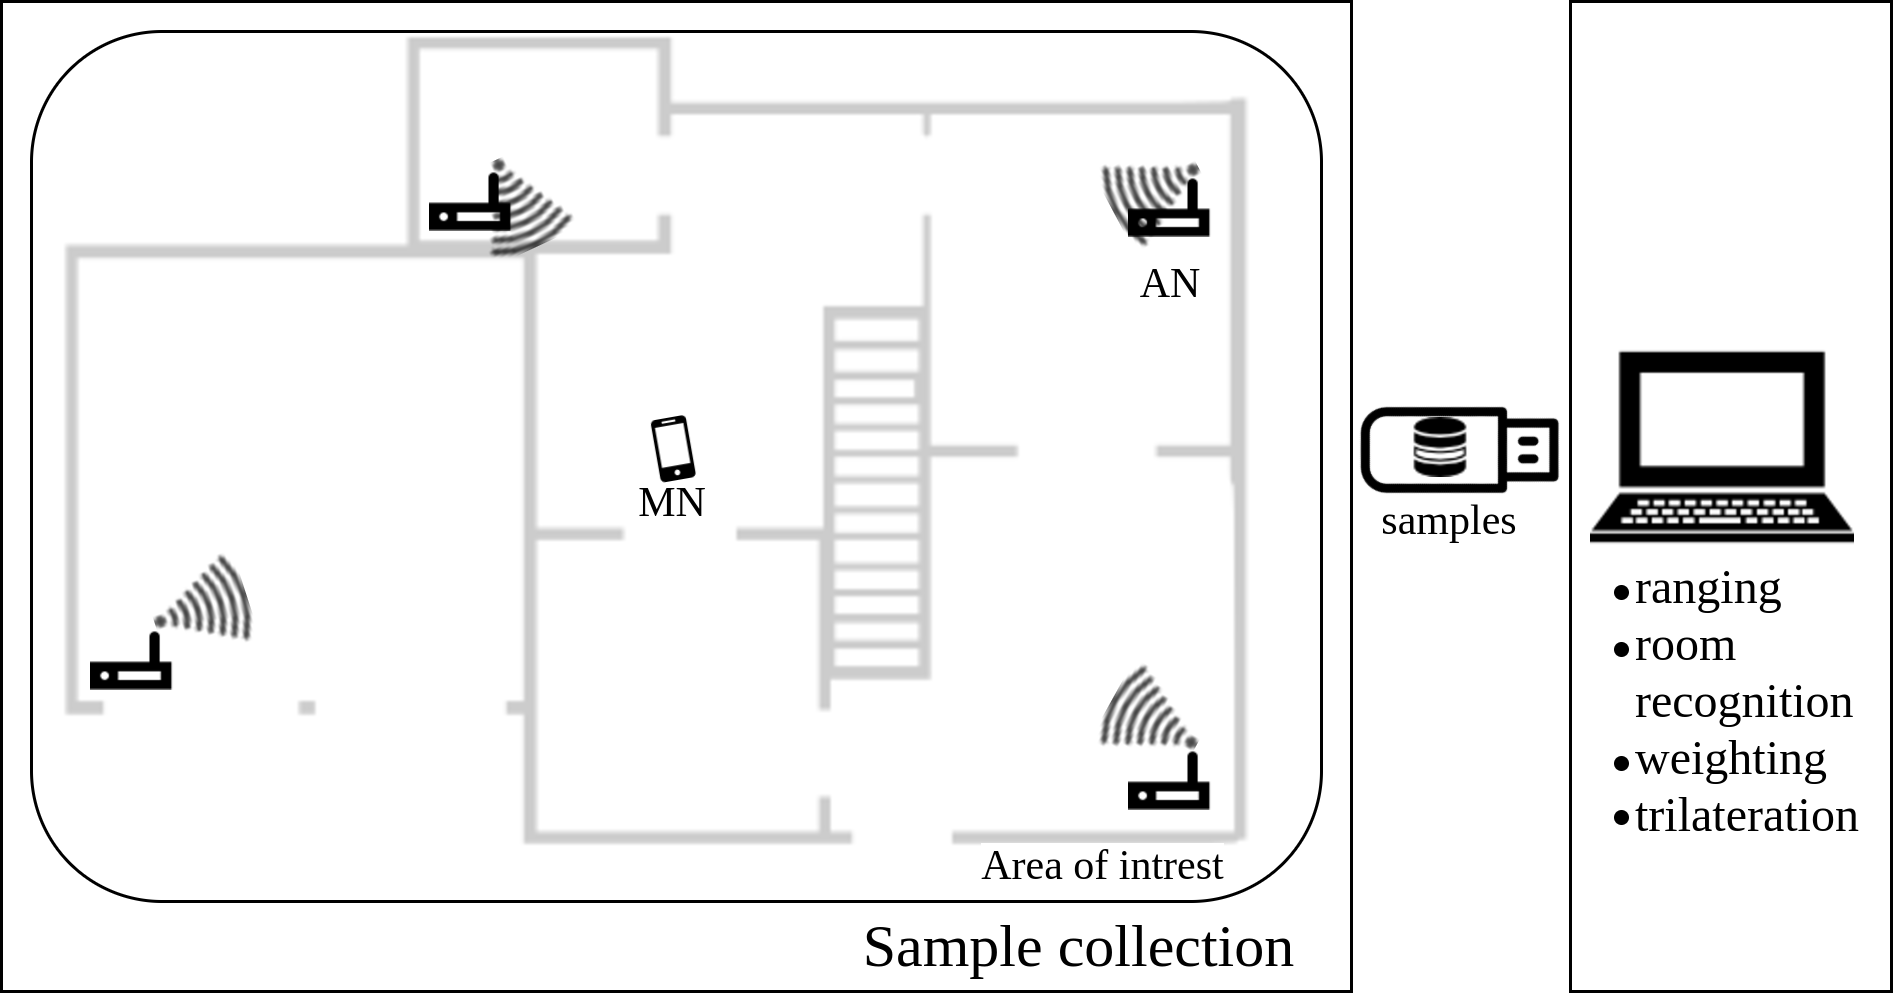
\includegraphics[width=\textwidth]{Figures/SystemImplementationOverview}
\decoRule
\caption[localization system overview]{Diagram of the test bed implementation}
\label{fig:existingApproach}
\end{figure}

This test bed implementation splits the system into an online \red{(collecting samples)} and offline \red{(calculations on the computer)} part. This allows easily try out and empirically compare different configurations of the localisation system under the exact same conditions.

The set-up of this test bed comprises both hardware and software specific configurations for each component. The remainder of this section details these configurations.

\section{Hardware Set-up}

This set-up requires three different kinds of machines. One for the AN, another for the MN and a computer. \red{There are no special requirements for the computer it only has to be able to execute Java code.}

For the AN and MN the following hardware was employed:

\paragraph{Anchor Nodes}
The commercial Wi-Fi access points used as anchor nodes are of the model D-Link D-635 and D-2553. They are set-up with a beacon period of 100ms and broadcast on the 2.4 GHz frequency band.

\paragraph{Mobile Node}

The mobile node is an android smartphone of the model \emph{One Plus One}. It has the following specifications:

\begin{itemize}
\item \textbf{OS:} Android 5.1
\item \textbf{Processor:} 2.5GHz Quad-core CPU
\item \textbf{WiFi module:} Qualcomm WCN3680 802.11ac/FM/BT 4.0 Combo Chip 
\item \textbf{Internal sensors:} accelerometer, magnetometer, gyroscope, proximity, ambient light
\item \textbf{Memory:} 3 GB RAM
\end{itemize}

The WiFi module and the magnetometer are used to collect the samples.


\section{Software Set-up}

\subsection{Sample collection}

The samples are collected on the smartphone using a small application written for this purpose.

The samples consist of:
\begin{itemize}
\item \textbf{A label} eather indicating the room or the exact location where the sample was taken.
\item \textbf{A set of RSSI values}, one for each AN.
\item \textbf{The magnetic field strength} in \(\mu\)-Tesla along the devices x,y and z axis.
\end{itemize}

On android the WiFi module can not be accessed directly. Wi-Fi scans have to be initiated through the \code{AndroidAPI} and it only supports full scans\cite{brouwers2014incremental}. Full scans take longer so it is only possible to take one RSSI measurement every 1.5 seconds.

To collect one sample the application takes the average of five RSSI and magnetometer measurements, each spaced 2 seconds apart. The samples are then saved to a \code{.csv} file on the smartphones internal storage and later transferred to the computer.

\subsection{Offline set-up}

Training, testing and evaluation of the localization system is done offline on a computer using a collection of different tools. For this purpose the collected samples are grouped into training and testing datasets. First the models for ranging, room recognition and weighting are created. These are then imported into a Java program which read

\subsubsection*{Room Recognition}
\red{The SVM is trained with an automated script provided by the libSVM library. It generates a multiclass SVM model from the fingerprinting map using cross validation to determine the best value for C and gamma}.
\note{change to WEKA}

\subsubsection*{Ranging}
For the ranging model the \(\alpha, \beta\) parameters from equation \ref{eqn:non-linear path loss model} need to be determined for each AN. So in a spreadsheet the distance between the AN and the samples is calculated from the ranging data. This results in a list of distances and corresponding RSSI values. Matlabs function fit tool is then used to find the \(\alpha, \beta\)-values that best fit this data.
\note{Insert example image here}

As apparent in the example above, this non-linear path loss model is inaccurate with high RSSI values. To account for that the distances for these high values are set by hand.

\subsubsection*{Weighting}

The room weights are determined by hand in a spreadsheet based on the formal definition given in section \ref{WeightingModelDefinition}
\note{talk about implementation of dinamic factor in java}

\subsection{Testing the Models}